% Created 2016-02-18 Thu 13:38
\documentclass{article}
\usepackage[utf8]{inputenc}
\usepackage[T1]{fontenc}
\usepackage{fixltx2e}
\usepackage{graphicx}
\usepackage{grffile}
\usepackage{longtable}
\usepackage{wrapfig}
\usepackage{rotating}
\usepackage[normalem]{ulem}
\usepackage{amsmath}
\usepackage{textcomp}
\usepackage{amssymb}
\usepackage{capt-of}
\usepackage{hyperref}
\author{Taylor Foxhall}
\date{\today}
\title{Simple Line Drawing Algorithms}
\hypersetup{
 pdfauthor={Taylor Foxhall},
 pdftitle={Simple Line Drawing Algorithms},
 pdfkeywords={},
 pdfsubject={},
 pdfcreator={Emacs 24.5.1 (Org mode 8.3.3)}, 
 pdflang={English}}
\begin{document}

\maketitle

\section{Introduction}
\label{sec:orgheadline1}
In the field of computer graphics, there are two well-known algorithms used for drawing lines. We will compare
Brensenham's algorithm, the midpoint line algorithm, and OpenGL's implementation of line drawing.
\section{Brensenham Line Drawing}
\label{sec:orgheadline5}
\subsection{Idea}
\label{sec:orgheadline2}
Brensenham's algorithm chooses which pixel to draw based on an accumulated error. Assuming we're trying to draw
a line that is in the first octant of a graph, we can draw horizontally unless our error crosses a certain threshold,
then we increment y and subtract the accumulated error. Other lines in other octants can be handled by a simple
transformation (not shown below, but is included in the \href{main.cpp}{source file}.)
\subsection{Code Exposé}
\label{sec:orgheadline3}
\begin{verbatim}
void brensenham_line(int x0, int y0, int x1, int y1) {
  int dx = x1 - x0;
  int dy = y1 - y0;
  int y = y0;
  int decider = 2*dy - dx;

  glBegin(GL_POINTS);
  for (int x = x0; x <= x1; x++) {
    glVertex2i(x, y);
    decider += 2*dy;
    if (decider > 0) {
      y++;
      decider -= 2*dx;
    }
  }
  glEnd();
}
\end{verbatim}
\subsection{Demos}
\label{sec:orgheadline4}
\begin{figure}[htb]
\centering
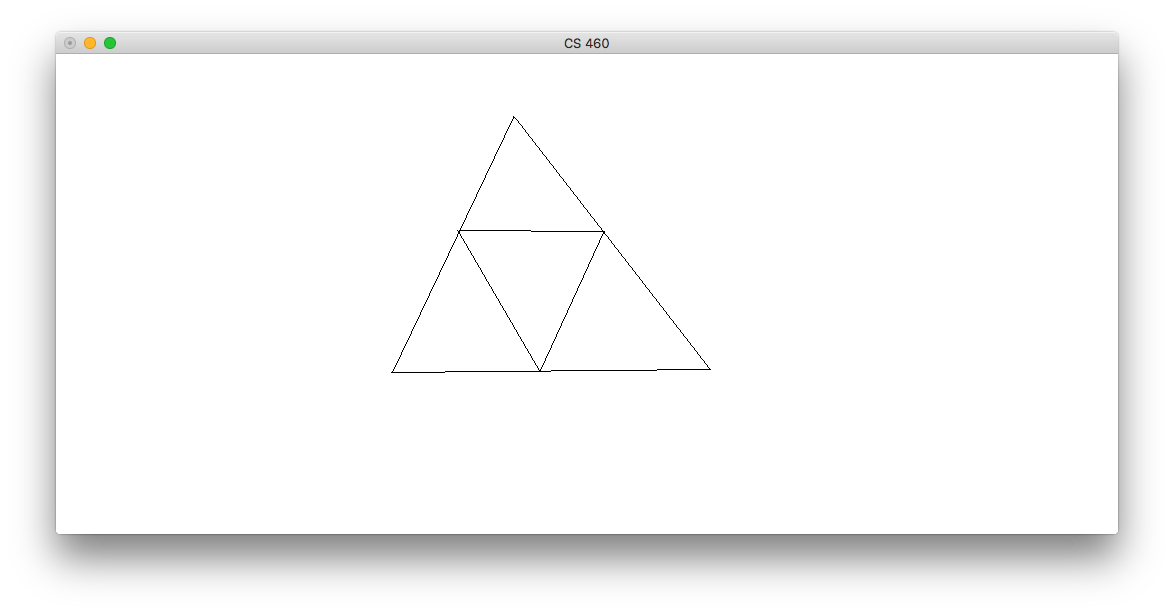
\includegraphics[width=.9\linewidth]{./img/a1_bren_basic.png}
\caption{A simple drawing using Brensenham's algorithm}
\end{figure}
\begin{figure}[htb]
\centering
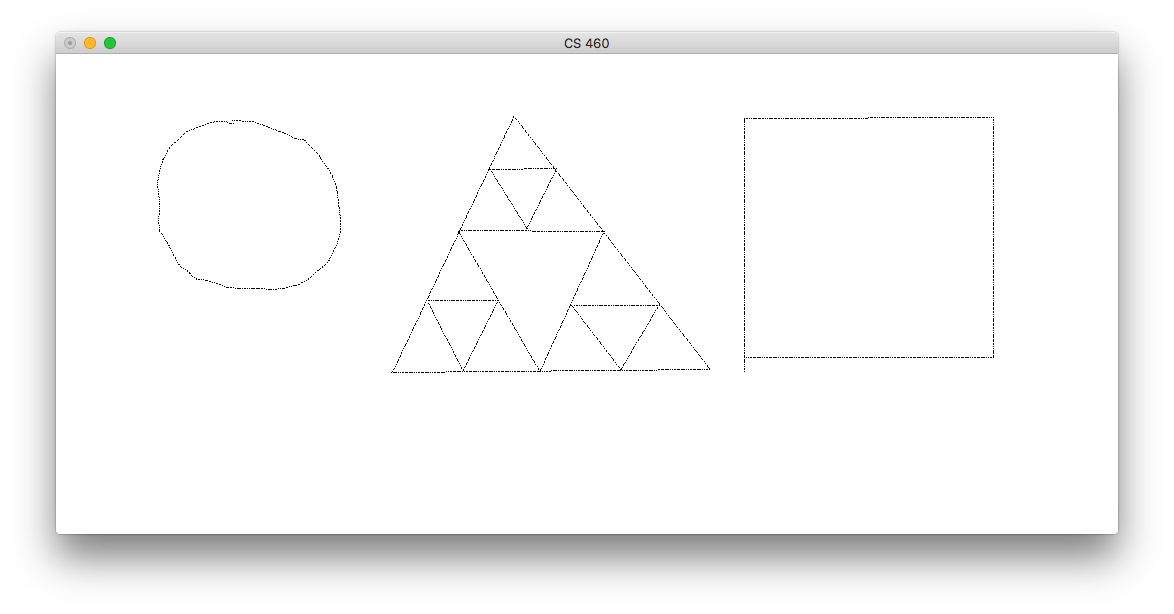
\includegraphics[width=.9\linewidth]{./img/a1_bren_stipple.png}
\caption{Line stippling with Brensenham's algorithm}
\end{figure}
\begin{figure}[htb]
\centering
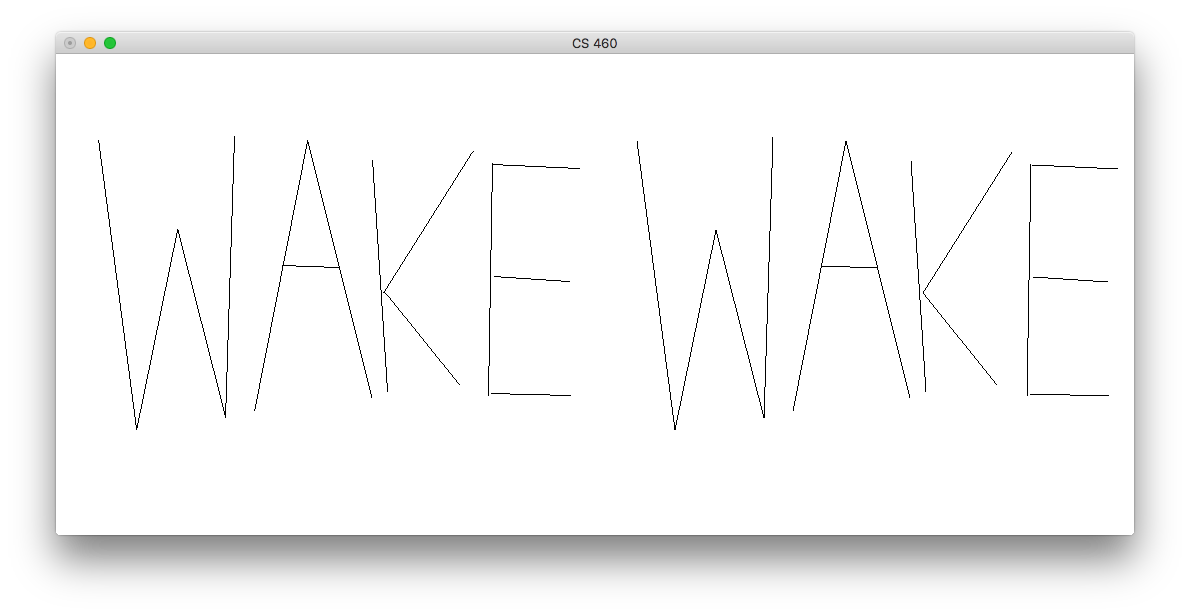
\includegraphics[width=.9\linewidth]{./img/a1_wake.png}
\caption{"WAKE" drawn with Brensenham's algorithm (left) vs. OpenGL's lines (right)}
\end{figure}
\section{Midpoint Line Drawing}
\label{sec:orgheadline9}
\subsection{Idea}
\label{sec:orgheadline6}
This algorithm tries to improve upon Brensenham by substituting the error accumulator
for an approximation of the line function and compares it with its location of the
midpoint of the eastern pixel and the northeastern pixel. The algorithm fills in
whatever pixel is closer to the approximation. The octant switching in Brensenham's
algorithm still applies.
\subsection{Code Exposé}
\label{sec:orgheadline7}
\begin{verbatim}
void midpoint_line(int x0, int y0, int x1, int y1) {
  int dx = x1 - x0;
  int dy = y1 - y0;
  int y = y0;
  int decider = 2*dy - dx;
  int inc_e = 2*dy;
  int inc_ne = 2*(dy - dx);

  glBegin(GL_POINTS);
  for (int x = x0; x <= x1; x++) {
      glVertex2i(x, y);
    if (decider > 0) {
      decider += inc_ne;
      y++;
    }
    else {
      decider += inc_e;
    }
  }
  glEnd();
}
\end{verbatim}
\subsection{Demos}
\label{sec:orgheadline8}
\begin{figure}[htb]
\centering
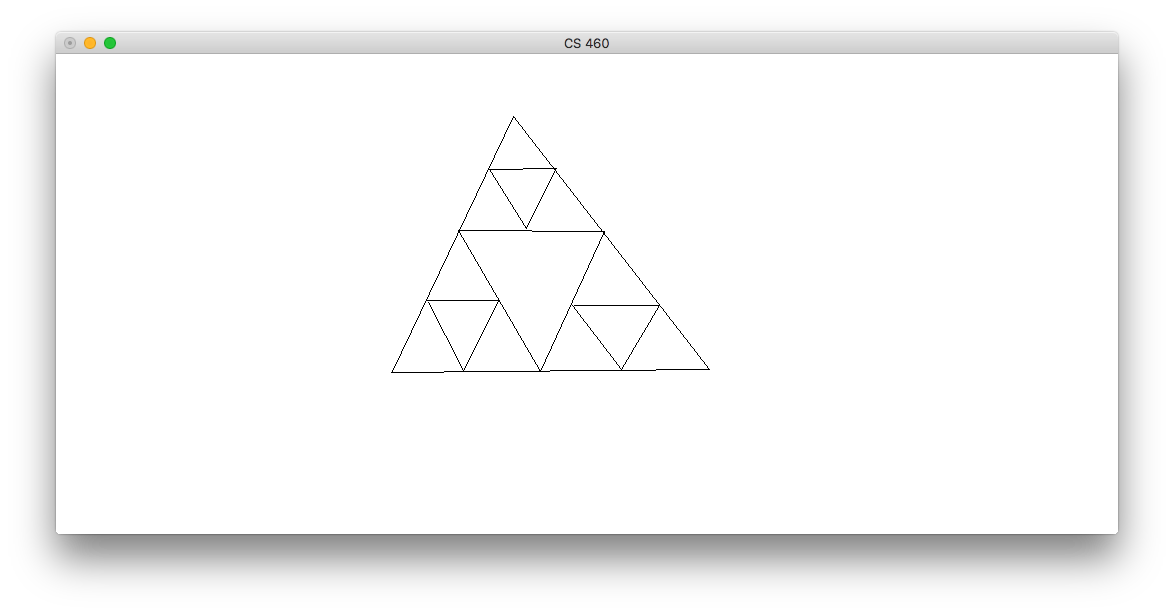
\includegraphics[width=.9\linewidth]{./img/a1_midpt_basic.png}
\caption{A simple drawing using the Midpoint algorithm}
\end{figure}
\begin{figure}[htb]
\centering
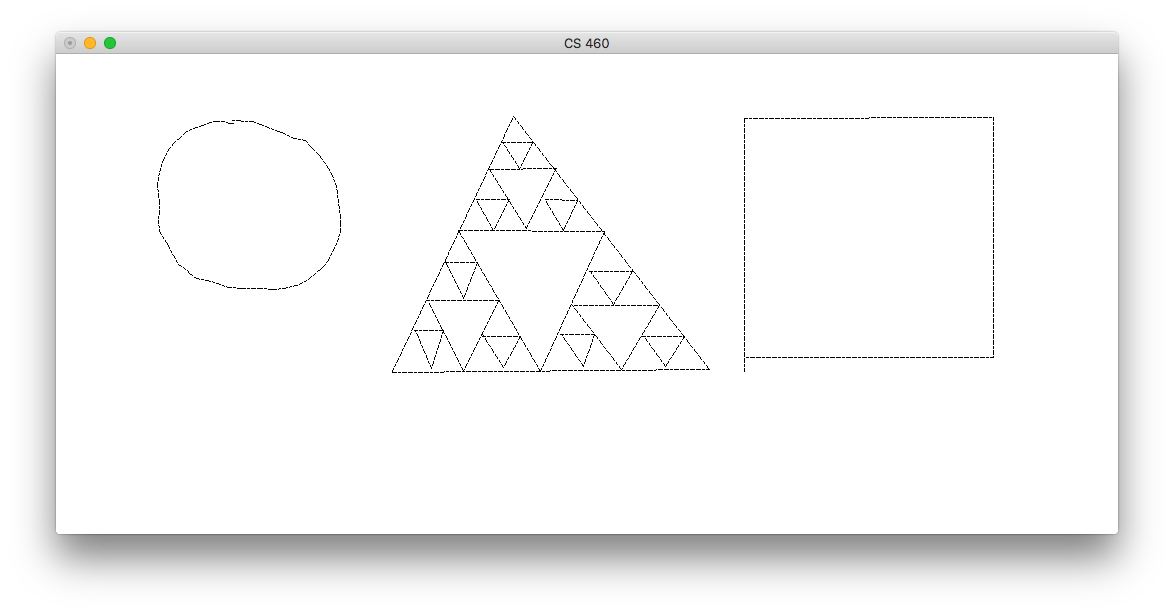
\includegraphics[width=.9\linewidth]{./img/a1_midpt_stipple.png}
\caption{Line stippling with the Midpoint algorithm}
\end{figure}
\begin{figure}[htb]
\centering
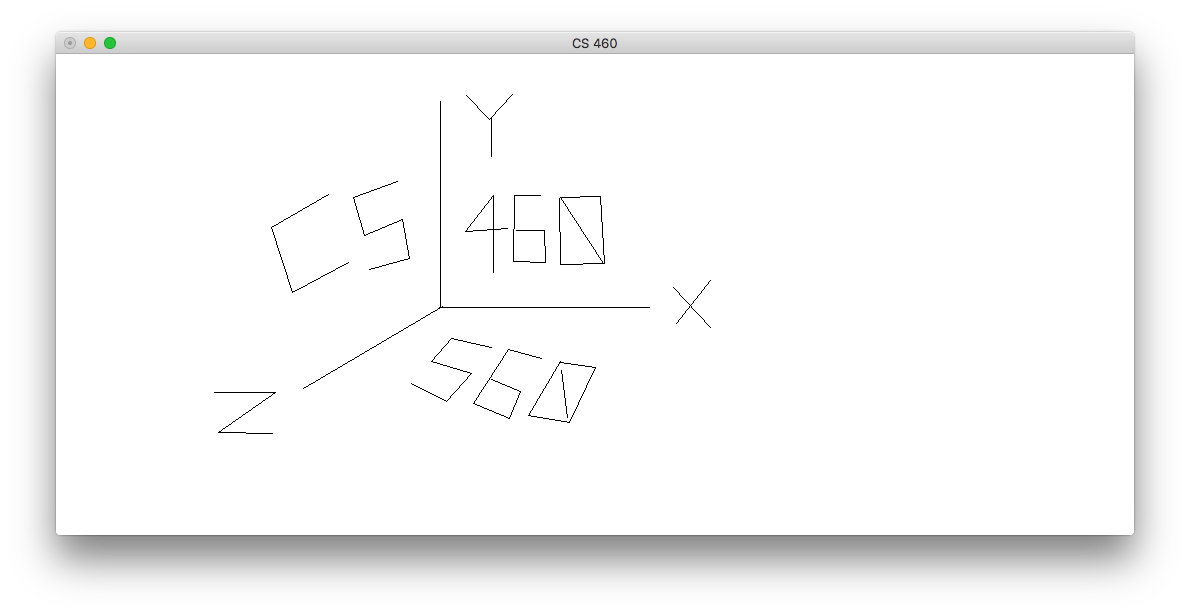
\includegraphics[width=.9\linewidth]{./img/a1_coord.png}
\caption{A coordinate system drawn with the Midpoint algorithm}
\end{figure}
\end{document}